% This file was created with matplot2tikz v0.5.4.
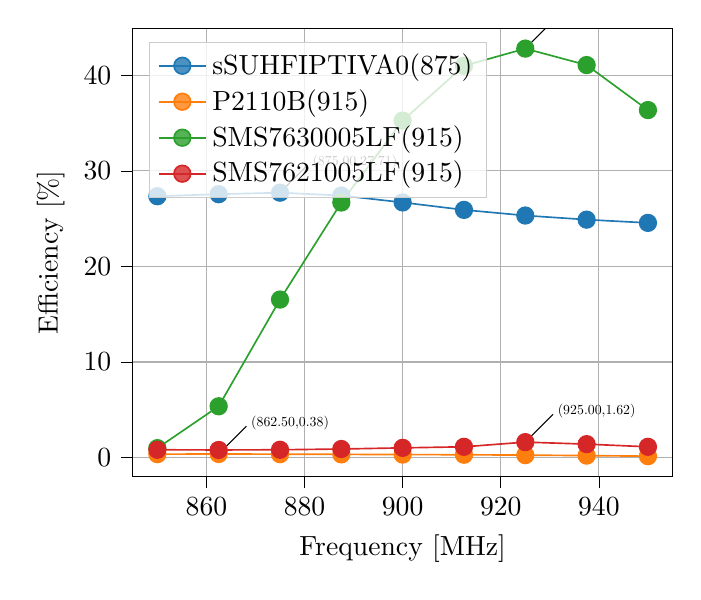
\begin{tikzpicture}

\definecolor{crimson2143940}{RGB}{214,39,40}
\definecolor{darkgray176}{RGB}{176,176,176}
\definecolor{darkorange25512714}{RGB}{255,127,14}
\definecolor{forestgreen4416044}{RGB}{44,160,44}
\definecolor{lightgray204}{RGB}{204,204,204}
\definecolor{steelblue31119180}{RGB}{31,119,180}

\begin{axis}[
legend cell align={left},
legend style={
  fill opacity=0.8,
  draw opacity=1,
  text opacity=1,
  at={(0.03,0.97)},
  anchor=north west,
  draw=lightgray204
},
tick align=outside,
tick pos=left,
x grid style={darkgray176},
xlabel={Frequency [MHz]},
xmajorgrids,
xmin=845, xmax=955,
xtick style={color=black},
y grid style={darkgray176},
ylabel={Efficiency [\%]},
ymajorgrids,
ymin=-1.9815, ymax=44.9115,
ytick style={color=black}
]
\addplot [semithick, steelblue31119180, mark=*, mark size=3, mark options={solid}]
table {%
850 27.34
862.5 27.55
875 27.71
887.5 27.41
900 26.69
912.5 25.91
925 25.32
937.5 24.89
950 24.55
};
\addlegendentry{sSUHFIPTIVA0(875)}
\addplot [semithick, darkorange25512714, mark=*, mark size=3, mark options={solid}]
table {%
850 0.36
862.5 0.38
875 0.36
887.5 0.34
900 0.32
912.5 0.3
925 0.26
937.5 0.21
950 0.15
};
\addlegendentry{P2110B(915)}
\addplot [semithick, forestgreen4416044, mark=*, mark size=3, mark options={solid}]
table {%
850 0.99
862.5 5.37
875 16.53
887.5 26.68
900 35.25
912.5 40.98
925 42.78
937.5 41.06
950 36.35
};
\addlegendentry{SMS7630005LF(915)}
\addplot [semithick, crimson2143940, mark=*, mark size=3, mark options={solid}]
table {%
850 0.82
862.5 0.8
875 0.82
887.5 0.9
900 1.02
912.5 1.13
925 1.62
937.5 1.41
950 1.13
};
\addlegendentry{SMS7621005LF(915)}
\draw[->,draw=black] (axis cs:875,27.71) ++(10pt,10pt) -- (axis cs:875,27.71);
\draw (axis cs:875,27.71) ++(10pt,10pt) node[
  scale=0.5,
  anchor=base west,
  text=black,
  rotate=0.0
]{(875.00,27.71)};
\draw[->,draw=black] (axis cs:862.5,0.38) ++(10pt,10pt) -- (axis cs:862.5,0.38);
\draw (axis cs:862.5,0.38) ++(10pt,10pt) node[
  scale=0.5,
  anchor=base west,
  text=black,
  rotate=0.0
]{(862.50,0.38)};
\draw[->,draw=black] (axis cs:925,42.78) ++(10pt,10pt) -- (axis cs:925,42.78);
\draw (axis cs:925,42.78) ++(10pt,10pt) node[
  scale=0.5,
  anchor=base west,
  text=black,
  rotate=0.0
]{(925.00,42.78)};
\draw[->,draw=black] (axis cs:925,1.62) ++(10pt,10pt) -- (axis cs:925,1.62);
\draw (axis cs:925,1.62) ++(10pt,10pt) node[
  scale=0.5,
  anchor=base west,
  text=black,
  rotate=0.0
]{(925.00,1.62)};
\end{axis}

\end{tikzpicture}
